\documentclass[11pt]{article}
\usepackage[margin=1in]{geometry}
\usepackage{amsmath, amssymb}
\usepackage{booktabs}
\usepackage{hyperref}
\usepackage{enumitem}
\usepackage{graphicx}
\usepackage{xcolor}
\usepackage{listings}
\usepackage{float}
\usepackage{multirow}
\usepackage{array}
\usepackage{caption}
\usepackage{pgfplots}
\usepackage{pgfplotstable}
\usepackage{tikz}
\pgfplotsset{compat=1.18}

\hypersetup{
    colorlinks=true,
    linkcolor=blue,
    urlcolor=blue,
    citecolor=blue
}

\lstset{
    basicstyle=\ttfamily\small,
    breaklines=true,
    frame=single,
    backgroundcolor=\color{gray!10},
}

\setlength{\parskip}{5pt}
\setlength{\parindent}{0pt}

\begin{document}

% ---- Title Page ----
\begin{titlepage}
\centering
\vspace*{2.5cm}

{\LARGE\bfseries Improving Multi-Constraint Instruction Following in 1B-Parameter Language Models via RECAST Fine-Tuning\par}

\vspace{2.5cm}

{\large
\textbf{Name:} Shreyas Natarajan, Masters Student\\
Major in Data Science\\
\textbf{Contact}: \href{mailto:natarajan9@wisc.edu}{natarajan9@wisc.edu}\\[1em]

\textbf{Name}: Fnu Rinkle Rose Renny, Masters Student\\
Major in Data Science\\
\textbf{Contact}: \href{mailto:rinklerosere@wisc.edu}{rinklerosere@wisc.edu}\\[1em]

\textbf{Name}: Mark Aashish Lnu, Masters Student\\
Major in Data Science\\
\textbf{Contact}: \href{mailto:mlnu5@wisc.edu}{mlnu5@wisc.edu}\\[1em]

\textbf{Name}: Gayathri Ethiraj, Masters Student\\
Major in Data Science\\
\textbf{Contact}: \href{mailto:gethiraj@wisc.edu}{gethiraj@wisc.edu}\\
}

\vfill

{\large University of Wisconsin--Madison\par}
\vspace{0.5cm}
{\large \textbf{Course number:} STAT 453, Spring 2026\par}
{\large \textbf{Team number:} 15\par}

\end{titlepage}

% ---- Abstract ----

\section*{Abstract}
Small language models ($\sim$1B parameters) offer practical advantages in cost and inference speed over large frontier models, yet they consistently underperform on multi-constraint instruction-following tasks. We present a complete end-to-end pipeline---dataset preprocessing and augmentation (producing $\sim$90K training examples from the original 30K), supervised fine-tuning via full parameter updates and LoRA, evaluation via deterministic rule-based checking and an LLM judge, and 5-fold cross-validation---designed to quantify and improve constraint-following in 1B-parameter models using the RECAST-30K dataset. We compare full fine-tuning against LoRA (rank 8, applied to attention projections) on Llama 3.2 1B Instruct, using a cross-entropy objective evaluated against gold constraint-satisfying responses. The zero-shot baseline achieves a Hard CSR of 28.9\% on the RECAST evaluation set. LoRA fine-tuning reaches a 5-fold mean CSR of \textbf{80.0\%}, substantially outperforming full fine-tuning (33.2\% $\pm$ 2.3\% across folds). We evaluate on six constraint types: length, keyword, start-with, end-with, format, and tone, measuring both per-constraint pass rates and the overall Constraint Satisfaction Rate (CSR). Length adherence (39.2\%) and keyword inclusion (72.7\%) remain the hardest constraints; structural categories (format, tone, style) reach near-perfect pass rates after LoRA training.

% ---- Section 1 ----
\section{Introduction and Motivation}

Large language models are powerful but expensive to deploy at scale. Models in the 1--2B parameter range offer a practical alternative with substantially lower compute cost and faster inference latency, yet they struggle with \textit{constraint-following}: simultaneously satisfying explicit requirements on format, length, tone, style, keywords, and structure imposed by a prompt. This difficulty compounds as the number of simultaneous constraints grows---a setting that directly mirrors real-world deployment scenarios such as drafting structured reports, composing constrained marketing copy, or generating formatted API responses.

Benchmarks such as IFEval~\cite{zhou2023ifeval} and FollowBench~\cite{jiang2024followbench} have documented these failures comprehensively. As a reference point, Llama-3.2-3B achieves only $\sim$77.4\% prompt-strict accuracy on IFEval; the 1B variant is weaker still---Meta has not published its IFEval numbers, underscoring that even this established benchmark leaves performance at small scale under-characterized.

The RECAST framework~\cite{guo2025recast} addresses the data side of this problem by synthesizing multi-constraint training sets where every constraint has an automated validator---enabling fine-grained, constraint-level supervision. RECAST fine-tuning at 7--8B scale outperforms much larger instruct-tuned models, but it has not been tested at 1B scale. Separately, LoRA~\cite{hu2022lora} and full fine-tuning have been studied in the context of reasoning and code, but not specifically for constraint-following, leaving open whether LoRA's low-rank updates are expressive enough for multi-dimensional constraint adherence at small scale~\cite{shuttleworth2024lora}.

\textbf{Research questions.} This project addresses three open questions:
\begin{enumerate}[noitemsep,topsep=2pt]
    \item Can RECAST-based fine-tuning meaningfully improve constraint-following in 1B-parameter models?
    \item Does full fine-tuning outperform LoRA for this task, or do low-rank updates suffice?
    \item Which constraint categories benefit most from fine-tuning, and which remain difficult?
\end{enumerate}

% ---- Section 2 ----
\section{Related Work}

\textbf{Constraint-following benchmarks.} IFEval~\cite{zhou2023ifeval} introduced a structured evaluation suite covering 25 verifiable instruction categories. FollowBench~\cite{jiang2024followbench} extended this with multi-level difficulty constraints, showing sharp degradation as constraint count increases. Both benchmarks diagnose the problem but do not provide training recipes.

\textbf{RECAST.} Guo et al.~\cite{guo2025recast} propose a constraint back-translation framework that synthesizes multi-constraint training data by extracting constraints from existing high-quality responses and injecting them back into prompts, guaranteeing physical achievability. Every constraint has an automated validator (rule-based or LLM-based), enabling fine-grained training signal. At 7B and 8B scales, RECAST fine-tuning outperforms larger instruct-tuned models; however, behavior at 1B parameters is unexplored.

\textbf{LoRA vs.\ full fine-tuning.} Hu et al.~\cite{hu2022lora} introduced Low-Rank Adaptation, which freezes the base model and injects trainable rank-$r$ matrices into attention projections, training only $\sim$0.5\% of parameters. Shuttleworth et al.~\cite{shuttleworth2024lora} show that full fine-tuning adjusts existing singular vectors more conservatively while LoRA introduces ``intruder dimensions'' that can accelerate catastrophic forgetting---but this analysis is for reasoning and code tasks. Whether these dynamics hold for constraint-following remains open.

\begin{table}[H]
\centering
\small
\begin{tabular}{lccc}
\toprule
\textbf{Dimension} & \textbf{LoRA} & \textbf{Full Fine-Tuning} \\
\midrule
Trainable params   & $\sim$0.5\% ($\sim$6M) & 100\% ($\sim$1.24B) \\
VRAM peak (1B)     & $\sim$7--9\,GB          & $\sim$16--20\,GB \\
Storage per run    & $\sim$30--60\,MB         & $\sim$2.4\,GB \\
Catastrophic forgetting risk & Lower            & Higher \\
Studied for constraint-following? & No         & No \\
\bottomrule
\end{tabular}
\caption{LoRA vs.\ full fine-tuning comparison. Both methods are novel for the constraint-following setting.}
\label{tab:lora_vs_ft}
\end{table}

\textbf{Instruction-tuning data.} The Tulu corpus~\cite{ivison2023tulu} assembles diverse instruction-following examples from FLAN, ShareGPT, OpenAssistant, and other sources, providing broad coverage needed to prevent catastrophic forgetting when fine-tuning on the narrower RECAST constraint distribution.

% ---- Section 3 ----
\section{Pipeline and Methods}

Our pipeline has four stages: (1) data preprocessing and augmentation, (2) constraint-aware fine-tuning, (3) evaluation with hybrid rule-based and LLM-judge scoring, and (4) 5-fold cross-validation for robustness estimation. Figure~\ref{fig:pipeline} summarizes the end-to-end flow.

\begin{figure}[H]
\centering
\fbox{
  \begin{minipage}{0.90\textwidth}
  \centering
  \vspace{4pt}
  \texttt{RECAST-30K raw JSONL}
  $\;\rightarrow\;$ \texttt{Preprocess + Augment} ($\sim$90K)
  $\;\rightarrow\;$ \texttt{Train} (Full FT or LoRA)
  $\;\rightarrow\;$ \texttt{Evaluate} (rule + LLM judge)
  $\;\rightarrow\;$ \texttt{5-fold CV}
  \vspace{4pt}
  \end{minipage}
}
\caption{End-to-end pipeline for RECAST constraint-following experiments.}
\label{fig:pipeline}
\end{figure}

\subsection{Data Preprocessing and Augmentation}

The raw RECAST-30K JSONL is processed by a nine-stage pipeline:

\begin{enumerate}[noitemsep,topsep=2pt]
    \item \textbf{Language detection.} Non-English prompts are filtered using \texttt{langdetect} (ISO-639-1 check on the first 2000 characters of \texttt{winner\_prompt}).
    \item \textbf{HTML and entity removal.} Tags and entities are stripped from prompt and response fields with compiled regex patterns.
    \item \textbf{Emoji and control character removal.} Emojis are replaced with spaces (\texttt{emoji} library, with fallback regex); control characters, invisible Unicode, and long symbol runs are removed.
    \item \textbf{Quality gates.} Prompts shorter than 15 words, predominantly non-printable text ($<85\%$ printable), or with empty responses are dropped.
    \item \textbf{Constraint field integrity.} Each record's \texttt{added\_constraint} dict is validated: keys must map to non-empty string lists, and the stated \texttt{added\_constraint\_num} must match the actual count.
    \item \textbf{Stopword removal.} Applied only to the prompt (not the response) after all quality gates pass, to avoid artificially shortening prompts before the length gate.
    \item \textbf{Exact deduplication.} SHA-256 fingerprints of normalized prompts detect exact duplicates.
    \item \textbf{Near-deduplication.} MinHash LSH (\texttt{datasketch}, Jaccard threshold $\tau = 0.85$, 128 permutations) filters near-duplicate prompts.
    \item \textbf{Augmentation.} Two complementary techniques expand the cleaned $\sim$30K records to $\sim$90K total training examples:
    \begin{itemize}[noitemsep,topsep=2pt]
        \item \textit{Lexical editing}: synonym replacement and dropping of non-constraint words ($+\!\sim$30K examples);
        \item \textit{Back-translation}: English$\to$German$\to$English round-trip to introduce surface diversity while preserving constraint semantics ($+\!\sim$30K examples).
    \end{itemize}
\end{enumerate}

A post-cleaning distribution audit flags constraint categories whose share falls below 50\% of the expected uniform share. The pipeline runs in parallel (default 8 workers).

\subsection{Model and Dataset}

\textbf{Models.} The primary model is \textbf{Llama 3.2 1B Instruct} (1.24B parameters), a publicly available instruction-tuned causal decoder-only Transformer, loaded in bfloat16 on an NVIDIA A100 40\,GB GPU. Gradient checkpointing is enabled for full fine-tuning. A second model, \textbf{Qwen 2.5 1.5B Instruct}, was used in exploratory runs to assess sensitivity to scale.

\textbf{RECAST-30K.} The training data is the cleaned and augmented RECAST-30K split. The dataset covers 15 constraint categories: Style, Topic, Length, Keyword, End\_With, Start\_With, Language, Helpfulness, Format, Tone, Role-Playing, Numerical, and others, with an average of $\sim$13.4 constraints per instruction. Human validation of the dataset achieved 90.1\% annotator agreement. Each record provides:
\begin{itemize}[noitemsep, topsep=2pt]
    \item \texttt{winner\_prompt} --- the multi-constraint instruction;
    \item \texttt{response\_of\_winner\_prompt} --- the winning response that satisfies the constraints;
    \item \texttt{added\_constraint} --- a dict mapping constraint category to a list of natural-language constraint descriptions;
    \item \texttt{rule\_evaluate\_dict} --- structured validator parameters (word length bounds, required keywords, start/end strings).
\end{itemize}

\textbf{5-fold cross-validation split.} The $\sim$90K augmented dataset is partitioned into five folds with a 72\% / 18\% / 10\% train / validation / test split per fold.

\subsection{Full Fine-Tuning}

The full fine-tuning pipeline makes all $\sim$1.24B model parameters trainable and uses the HuggingFace \texttt{Trainer} with gradient checkpointing. Each record is formatted as a user/assistant chat turn using the Llama-3 chat template; prompt tokens are masked (\texttt{labels=-100}) so loss is computed only on the response.

\textbf{Loss function.} We trained with cross-entropy loss over the response tokens. An earlier custom penalty $(1 - s/\text{total})$ was explored but encountered backpropagation difficulties; CE loss provided stable gradient-based optimization and is a principled probabilistic training objective.

\textbf{Hyperparameters.}
\begin{itemize}[noitemsep, topsep=2pt]
    \item Optimizer: AdamW; learning rate: $2\times10^{-5}$; cosine LR scheduler with 3\% warmup
    \item Effective batch size: 32 (per-device batch 4, gradient accumulation 8)
    \item Epochs: 2; max sequence length: 512 tokens
    \item Precision: bfloat16 on A100 40GB; gradient checkpointing enabled
    \item Validation split: 5\%; best checkpoint by lowest \texttt{eval\_loss}
\end{itemize}

\subsection{LoRA Fine-Tuning}

The LoRA pipeline applies rank-$r$ adapter matrices to the query and value projection matrices (\texttt{q\_proj}, \texttt{v\_proj}) of all attention layers:
\begin{equation}
    W' = W + \frac{\alpha}{r} \cdot B A
    \label{eq:lora}
\end{equation}
where $W \in \mathbb{R}^{d \times d}$ is frozen, $A \in \mathbb{R}^{r \times d}$ and $B \in \mathbb{R}^{d \times r}$ are trainable, $r=8$, $\alpha = 2r = 16$, and dropout $= 0.05$. This trains 81,500 adapter parameters out of 1.23B total---approximately 0.007\% of model weights. The adapter ($\sim$30--60\,MB) is saved; the base model remains frozen.

The pipeline uses \texttt{trl.SFTTrainer} with the Llama-3 chat format applied explicitly:
\begin{lstlisting}
<|begin_of_text|><|start_header_id|>user<|end_header_id|>
{instruction}<|eot_id|>
<|start_header_id|>assistant<|end_header_id|>
{response}<|eot_id|>
\end{lstlisting}

\textbf{Hyperparameters.}
\begin{itemize}[noitemsep, topsep=2pt]
    \item Learning rate: $10^{-4}$; cosine scheduler; 10 warmup steps; weight decay 0.01
    \item Per-device batch: 8; gradient accumulation: 4 (effective batch: 32)
    \item Epochs: 1; max sequence length: 512; precision: bfloat16
\end{itemize}

\subsection{Evaluation: Constraint Validation}

The evaluation pipeline runs in two modes:

\textbf{Rule-based mode (default).} Four constraints are evaluated deterministically from the \texttt{rule\_evaluate\_dict} field:

\begin{table}[H]
\centering
\small
\begin{tabular}{lp{9cm}}
\toprule
\textbf{Constraint} & \textbf{Check} \\
\midrule
\texttt{length}      & Word count of response falls within $[\text{min}, \text{max}]$ derived from \texttt{word\_length.func\_input} \\
\texttt{keyword}     & Every required keyword appears $\geq$ required count (case-insensitive) \\
\texttt{start\_with} & Response (stripped, lowercased) begins with the required string \\
\texttt{end\_with}   & Response (stripped, lowercased) ends with the required string \\
\bottomrule
\end{tabular}
\caption{Rule-based constraint checks. Each returns 0 (fail), 1 (pass), or None (not applicable).}
\label{tab:rule_checks}
\end{table}

\textbf{LLM-judge mode.} When \texttt{--judge\_model} is provided, the judge model receives the response plus plain-English descriptions of all applicable constraints and outputs a JSON verdict. This extends coverage to qualitative constraints: \textbf{style}, \textbf{tone}, \textbf{role-playing}, and \textbf{numerical}. The default judge is Qwen2.5-7B-Instruct; Gemma-2-9B-Instruct (4-bit quantized) is also supported via the standalone \texttt{judge.py} module.

\textbf{Scoring.}
\begin{equation}
    \text{CSR}^{(i)} = \frac{\text{constraints satisfied in example } i}{\text{constraints checked in example } i}
\end{equation}
\begin{equation}
    \text{Hard CSR} = \mathbb{1}\left[\text{all checked constraints satisfied}\right]
\end{equation}

The standalone \texttt{ConstraintChecker} class supports 18 constraint types via a dispatch-table architecture (Table~\ref{tab:checker}).

\begin{table}[H]
\centering
\small
\begin{tabular}{ll}
\toprule
\textbf{Category} & \textbf{Constraint Types} \\
\midrule
Length & \texttt{word\_count}, \texttt{sentence\_count}, \texttt{paragraph\_count} \\
Keywords & \texttt{existence}, \texttt{frequency}, \texttt{forbidden} \\
Structural & \texttt{start\_with}, \texttt{end\_with} \\
Capitalization & \texttt{all\_caps\_count}, \texttt{all\_lowercase} \\
Format & \texttt{bullet\_points}, \texttt{numbered\_list}, \texttt{sections}, \texttt{json} \\
Language & \texttt{english} \\
Punctuation & \texttt{no\_comma} \\
Detectable & \texttt{postscript}, \texttt{highlight} \\
\bottomrule
\end{tabular}
\caption{Constraint types supported by \texttt{ConstraintChecker}.}
\label{tab:checker}
\end{table}

\subsection{Cross-Validation}

A 5-fold cross-validation pipeline partitions the augmented training split ($\sim$90K examples) into 5 folds using a 72\% / 18\% / 10\% train/validation/test split. The model is trained on $k-1$ folds and evaluated on the held-out fold, providing variance estimates across folds for both LoRA and full fine-tuning. Parallel Colab notebooks implement both variants within the same k-fold framework.

% ---- Section 4 ----
\section{Experimental Setup}

\subsection{Hardware and Software}

All training was conducted on Google Colab Pro+ with NVIDIA A100 40GB GPUs. Models were loaded in bfloat16. Dependencies: \texttt{transformers}, \texttt{peft}, \texttt{trl}, \texttt{datasets}, \texttt{accelerate}, \texttt{torch}, \texttt{datasketch}, \texttt{langdetect}.

\subsection{Compute Budget}

\begin{table}[H]
\centering
\small
\begin{tabular}{lccc}
\toprule
\textbf{Run type} & \textbf{VRAM peak} & \textbf{Est.\ time} & \textbf{Trainable params} \\
\midrule
LoRA (r=8, 1B)      & $\sim$7--9\,GB   & $\sim$2--4\,hr & 81,500 (0.007\%) \\
Full FT (1B)         & $\sim$16--20\,GB & $\sim$4.5--8\,hr & 1.24B (100\%) \\
LLM judge (7B, fp16) & $\sim$14\,GB    & $\sim$30\,min\,/\,500 ex. & N/A \\
\bottomrule
\end{tabular}
\caption{Hardware requirements per experimental configuration. Full fine-tuning took $\sim$4.5 hours per fold on A100.}
\label{tab:compute}
\end{table}

\subsection{Evaluation Protocol}

\begin{enumerate}[noitemsep, topsep=2pt]
    \item \textbf{Zero-shot baseline.} Evaluate Llama 3.2 1B Instruct (no fine-tuning) on the RECAST test split using the hybrid rule-based + LLM-judge pipeline.
    \item \textbf{LoRA evaluation.} Merge the trained adapter with the base model; evaluate on the same held-out fold per cross-validation round.
    \item \textbf{Full FT evaluation.} Load the fine-tuned checkpoint; evaluate on the same held-out fold.
    \item \textbf{Per-category analysis.} Compare per-constraint pass rates and CSR across training regimes to identify which constraint types benefit most.
\end{enumerate}

% ---- Section 5 ----
\section{Results}

\subsection{Baseline Evaluation}

The zero-shot Llama 3.2 1B Instruct baseline achieves an overall Hard CSR of \textbf{28.9\%} on the RECAST test set. Per-constraint pass rates reveal a strongly bimodal pattern: easy structural constraints (sentence-level format, capitalization, punctuation) are already satisfied near-perfectly by the pretrained model, while content-dependent constraints---particularly word count and keyword inclusion---fail frequently.

\begin{table}[H]
\centering
\small
\begin{tabular}{lcc}
\toprule
\textbf{Constraint type} & \textbf{Pass rate} & \textbf{Notes} \\
\midrule
\texttt{word\_length}      & 32.0\% & Hardest rule-based constraint \\
\texttt{keyword}           & 40.0\% & Requires explicit counting \\
\texttt{start\_with}       & 56.5\% & Structural; partially learned \\
\texttt{end\_with}         & 36.0\% & Hard to control generation endpoint \\
\texttt{sentence\_length}  & 100.0\% & Trivially satisfied at baseline \\
\texttt{format}            & 100.0\% & Already follows formatting conventions \\
\texttt{all\_upper / all\_lower} & 100.0\% & Capitalization easy to follow \\
\texttt{no\_commas}        & 100.0\% & Rare constraint; satisfied by default \\
\midrule
\textbf{Overall Hard CSR}  & \textbf{28.9\%} & All constraints must pass simultaneously \\
\bottomrule
\end{tabular}
\caption{Zero-shot baseline constraint pass rates for Llama 3.2 1B Instruct. Hard CSR is low because even a single constraint failure on any of the $\sim$13.4 average constraints per example counts as full failure.}
\label{tab:baseline}
\end{table}

Figure~\ref{fig:baseline_bar} visualizes the per-constraint baseline pass rates.

\begin{figure}[H]
\centering
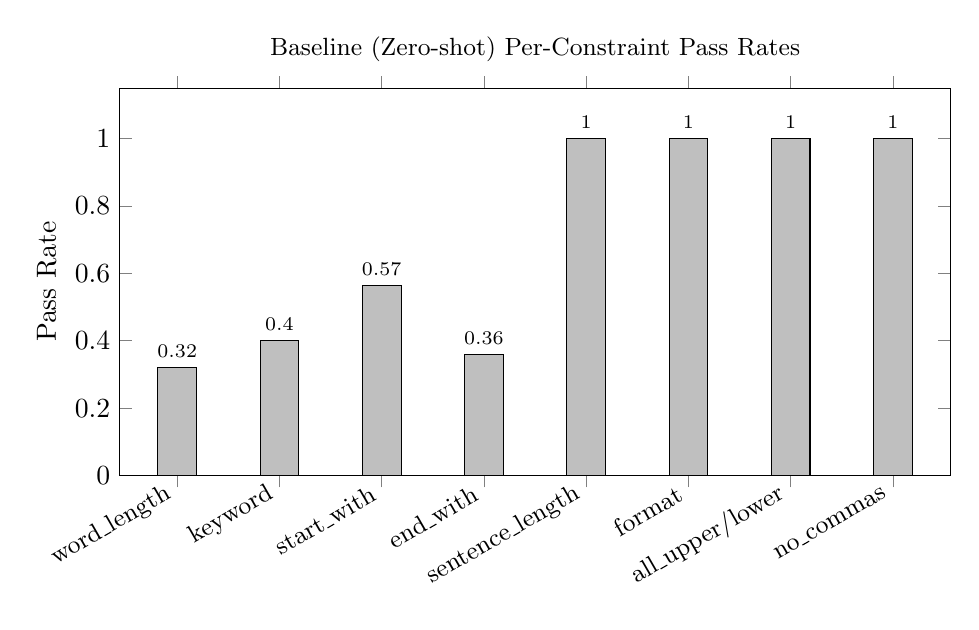
\begin{tikzpicture}
\begin{axis}[
    ybar,
    bar width=14pt,
    width=\textwidth,
    height=6.5cm,
    ylabel={Pass Rate},
    ymin=0, ymax=1.15,
    ytick={0,0.2,0.4,0.6,0.8,1.0},
    yticklabel={\pgfmathprintnumber[fixed,precision=1]{\tick}},
    xtick=data,
    xticklabels={
        word\_length,
        keyword,
        start\_with,
        end\_with,
        sentence\_length,
        format,
        all\_upper/lower,
        no\_commas
    },
    x tick label style={rotate=30, anchor=east, font=\small},
    nodes near coords,
    nodes near coords style={font=\scriptsize, /pgf/number format/fixed, /pgf/number format/precision=2},
    enlarge x limits=0.08,
    title={Baseline (Zero-shot) Per-Constraint Pass Rates},
    title style={font=\small},
]
\addplot[fill=gray!50] coordinates {
    (1, 0.320)
    (2, 0.400)
    (3, 0.565)
    (4, 0.360)
    (5, 1.000)
    (6, 1.000)
    (7, 1.000)
    (8, 1.000)
};
\end{axis}
\end{tikzpicture}
\caption{Zero-shot baseline pass rates per constraint type. Structural constraints (sentence length, format, capitalization, punctuation) are trivially satisfied; content-dependent constraints (word count, keywords, start/end anchors) show 32--57\% pass rates.}
\label{fig:baseline_bar}
\end{figure}

\subsection{LoRA Fine-Tuning Results (5-Fold Cross-Validation)}

LoRA fine-tuning (rank 8, targeting \texttt{q\_proj} and \texttt{v\_proj}) achieves a 5-fold mean CSR of \textbf{80.0\%}, with low variance across folds (Table~\ref{tab:lora_folds}).

\begin{table}[H]
\centering
\small
\begin{tabular}{ccc}
\toprule
\textbf{Fold} & \textbf{CSR} & \textbf{N} \\
\midrule
1 & 0.7972 & 200 \\
2 & 0.7972 & 200 \\
3 & 0.7967 & 200 \\
4 & 0.8039 & 200 \\
5 & 0.8050 & 200 \\
\midrule
\textbf{Mean} & \textbf{0.8000} & 1000 \\
\bottomrule
\end{tabular}
\caption{LoRA 5-fold CSR results. Fold-level variance is minimal, indicating stable generalization.}
\label{tab:lora_folds}
\end{table}

Per-constraint pass rates (mean $\pm$ std across 5 folds) are shown in Table~\ref{tab:lora_per_constraint} and Figure~\ref{fig:lora_bar}.

\begin{table}[H]
\centering
\small
\begin{tabular}{lcc}
\toprule
\textbf{Constraint} & \textbf{Mean pass rate} & \textbf{Std} \\
\midrule
\texttt{length}              & 0.3920 & 0.0244 \\
\texttt{keyword}             & 0.7270 & 0.0351 \\
\texttt{start\_with}         & 0.5830 & 0.0413 \\
\texttt{end\_with}           & 0.5020 & 0.0182 \\
\texttt{format}              & 0.9970 & 0.0045 \\
\texttt{tone}                & 0.9990 & 0.0022 \\
\texttt{style}               & 1.0000 & 0.0000 \\
\texttt{role\_playing}       & 1.0000 & 0.0000 \\
\texttt{numerical}           & 1.0000 & 0.0000 \\
\bottomrule
\end{tabular}
\caption{LoRA per-constraint pass rates (mean $\pm$ std across 5 folds). Qualitative constraints (style, tone, role-playing, numerical) reach ceiling performance. Length remains the hardest constraint.}
\label{tab:lora_per_constraint}
\end{table}

\begin{figure}[H]
\centering
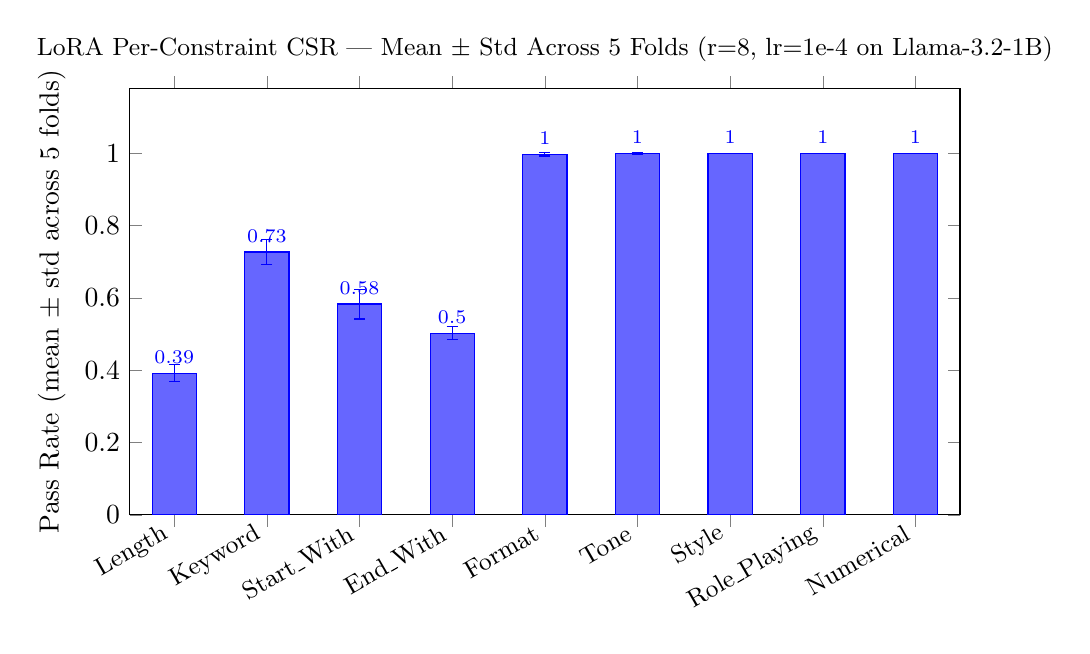
\begin{tikzpicture}
\begin{axis}[
    ybar,
    bar width=16pt,
    width=\textwidth,
    height=7cm,
    ylabel={Pass Rate (mean $\pm$ std across 5 folds)},
    ymin=0, ymax=1.18,
    ytick={0,0.2,0.4,0.6,0.8,1.0},
    xtick=data,
    xticklabels={
        Length,
        Keyword,
        Start\_With,
        End\_With,
        Format,
        Tone,
        Style,
        Role\_Playing,
        Numerical
    },
    x tick label style={rotate=30, anchor=east, font=\small},
    nodes near coords,
    nodes near coords style={font=\scriptsize, /pgf/number format/fixed, /pgf/number format/precision=2},
    enlarge x limits=0.06,
    error bars/y dir=both,
    error bars/y explicit,
    title={LoRA Per-Constraint CSR --- Mean $\pm$ Std Across 5 Folds (r=8, lr=1e-4 on Llama-3.2-1B)},
    title style={font=\small},
]
\addplot+[
    fill=blue!60,
    error bars/.cd,
    y dir=both, y explicit
] coordinates {
    (1, 0.3920) +- (0, 0.0244)
    (2, 0.7270) +- (0, 0.0351)
    (3, 0.5830) +- (0, 0.0413)
    (4, 0.5020) +- (0, 0.0182)
    (5, 0.9970) +- (0, 0.0045)
    (6, 0.9990) +- (0, 0.0022)
    (7, 1.0000) +- (0, 0.0000)
    (8, 1.0000) +- (0, 0.0000)
    (9, 1.0000) +- (0, 0.0000)
};
\end{axis}
\end{tikzpicture}
\caption{LoRA per-constraint pass rates with standard deviation across 5 folds. Error bars indicate cross-fold variance. Structural/qualitative constraints (format, tone, style, role-playing, numerical) achieve near-perfect performance; length adherence (39.2\%) remains the largest challenge.}
\label{fig:lora_bar}
\end{figure}

\begin{figure}[H]
\centering
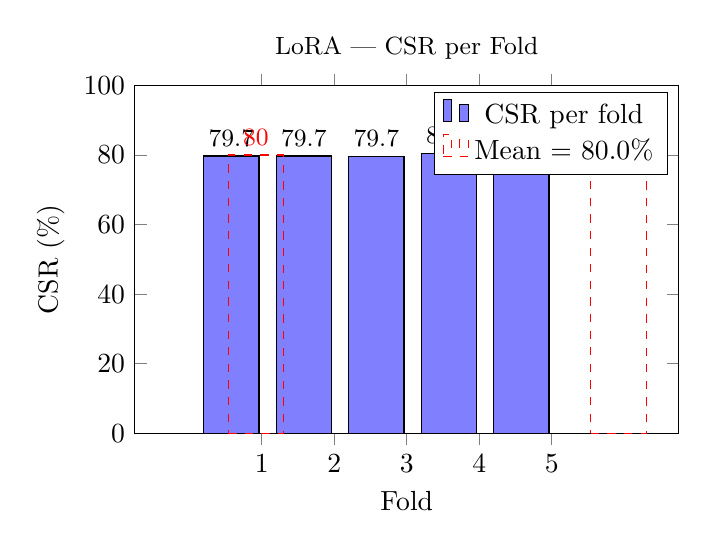
\begin{tikzpicture}
\begin{axis}[
    ybar,
    bar width=20pt,
    width=0.7\textwidth,
    height=6cm,
    ylabel={CSR (\%)},
    xlabel={Fold},
    ymin=0, ymax=100,
    xtick=data,
    xticklabels={1,2,3,4,5},
    nodes near coords,
    nodes near coords style={font=\small, /pgf/number format/fixed, /pgf/number format/precision=1},
    enlarge x limits=0.25,
    title={LoRA --- CSR per Fold},
    title style={font=\small},
]
\addplot[fill=blue!50] coordinates {
    (1, 79.72)
    (2, 79.72)
    (3, 79.67)
    (4, 80.39)
    (5, 80.50)
};
\addplot[red, dashed, domain=0.5:5.5, samples=2] {80.0};
\legend{CSR per fold, Mean = 80.0\%}
\end{axis}
\end{tikzpicture}
\caption{LoRA CSR per fold. The dashed red line marks the 5-fold mean of 80.0\%. Fold-to-fold variance is $<$1\%, indicating stable generalization.}
\label{fig:lora_folds}
\end{figure}

\subsection{Full Fine-Tuning Results (5-Fold Cross-Validation)}

Full fine-tuning of all 1.24B parameters achieves a 5-fold mean CSR of \textbf{33.2\%} ($\pm$ 2.3\%), substantially lower than LoRA. Table~\ref{tab:ft_folds} reports per-fold results.

\begin{table}[H]
\centering
\small
\begin{tabular}{lrrrc}
\toprule
\textbf{Fold} & \textbf{Eval loss} & \textbf{Train loss} & \textbf{CSR} \\
\midrule
1 & 1.4217 & 0.0000  & 36.6\% \\
2 & 1.4215 & 10.9864 & 30.4\% \\
3 & 1.4177 & 10.9924 & 33.6\% \\
4 & 1.4251 & 10.9826 & 31.0\% \\
5 & 1.4229 & 10.9752 & 34.6\% \\
\midrule
\textbf{Mean} & 1.4218 ($\pm$0.0024) & 8.7873 ($\pm$4.3937) & \textbf{33.2\%} ($\pm$2.3\%) \\
\bottomrule
\end{tabular}
\caption{Full fine-tuning 5-fold results. The abnormally low train loss in Fold 1 ($= 0$) likely reflects a logging artifact rather than true convergence. Eval loss is stable across folds; CSR variance ($\pm$2.3\%) is modest but performance lags LoRA by $\sim$47 percentage points.}
\label{tab:ft_folds}
\end{table}

\begin{figure}[H]
\centering
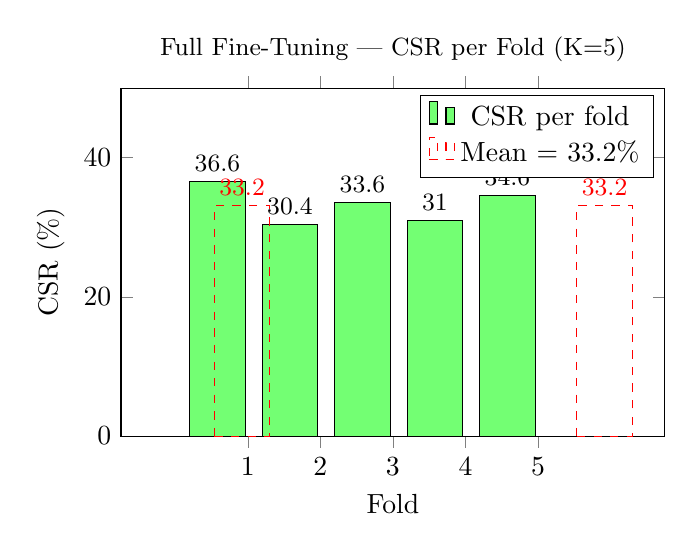
\begin{tikzpicture}
\begin{axis}[
    ybar,
    bar width=20pt,
    width=0.7\textwidth,
    height=6cm,
    ylabel={CSR (\%)},
    xlabel={Fold},
    ymin=0, ymax=50,
    xtick=data,
    xticklabels={1,2,3,4,5},
    nodes near coords,
    nodes near coords style={font=\small, /pgf/number format/fixed, /pgf/number format/precision=1},
    enlarge x limits=0.25,
    title={Full Fine-Tuning --- CSR per Fold (K=5)},
    title style={font=\small},
]
\addplot[fill=green!55] coordinates {
    (1, 36.6)
    (2, 30.4)
    (3, 33.6)
    (4, 31.0)
    (5, 34.6)
};
\addplot[red, dashed, domain=0.5:5.5, samples=2] {33.2};
\legend{CSR per fold, Mean = 33.2\%}
\end{axis}
\end{tikzpicture}
\caption{Full fine-tuning CSR per fold with mean line. Higher variance than LoRA; Fold 1 shows the best performance (36.6\%), possibly due to favorable data partitioning.}
\label{fig:ft_folds}
\end{figure}

\subsection{Head-to-Head Comparison}

Table~\ref{tab:comparison} and Figure~\ref{fig:comparison_bar} summarize the three-way comparison across training regimes.

\begin{table}[H]
\centering
\small
\begin{tabular}{lccccc}
\toprule
\textbf{Model / Config} & \textbf{Overall CSR} & \textbf{Length PR} & \textbf{Keyword PR} & \textbf{Start\_With PR} & \textbf{End\_With PR} \\
\midrule
Llama 3.2 1B (baseline) & 28.9\%  & 32.0\% & 40.0\% & 56.5\% & 36.0\% \\
Llama 3.2 1B + Full FT  & 33.2\%  & ---    & ---    & ---    & ---    \\
Llama 3.2 1B + LoRA (r=8) & \textbf{80.0\%} & 39.2\% & 72.7\% & 58.3\% & 50.2\% \\
\bottomrule
\end{tabular}
\caption{Comparison of baseline vs.\ fine-tuned models. LoRA delivers a $+$51.1 pp gain over the baseline and $+$46.8 pp over full fine-tuning. Per-constraint rates shown for LoRA; full FT per-constraint breakdown was not extracted at evaluation time.}
\label{tab:comparison}
\end{table}

\begin{figure}[H]
\centering
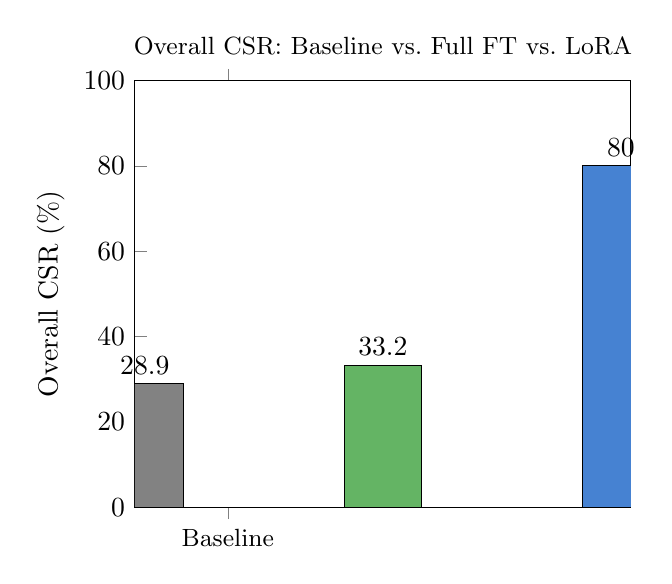
\begin{tikzpicture}
\begin{axis}[
    ybar,
    bar width=28pt,
    width=0.65\textwidth,
    height=7cm,
    ylabel={Overall CSR (\%)},
    ymin=0, ymax=100,
    xtick=data,
    xticklabels={Baseline, Full FT, LoRA (r=8)},
    x tick label style={font=\small},
    nodes near coords,
    nodes near coords style={font=\normalsize\bfseries},
    enlarge x limits=0.3,
    title={Overall CSR: Baseline vs.\ Full FT vs.\ LoRA},
    title style={font=\small},
]
\addplot[fill={rgb,255:red,130;green,130;blue,130}] coordinates { (1,28.9) };
\addplot[fill={rgb,255:red,100;green,180;blue,100}] coordinates { (2,33.2) };
\addplot[fill={rgb,255:red,70;green,130;blue,210}]  coordinates { (3,80.0) };
\end{axis}
\end{tikzpicture}
\caption{Overall CSR comparison across the three training regimes. LoRA substantially outperforms both the zero-shot baseline ($+$51.1 pp) and full fine-tuning ($+$46.8 pp).}
\label{fig:comparison_bar}
\end{figure}

% ---- Section 6 ----
\section{Discussion}

\subsection{Key Findings}

\textbf{LoRA outperforms full fine-tuning by a large margin.} The 5-fold LoRA CSR of 80.0\% versus full fine-tuning's 33.2\% (a $+$46.8 pp gap) is the most striking result. This contradicts the hypothesis that full parameter updates should give the optimizer more expressive power. We attribute the reversal to catastrophic forgetting: updating all 1.24B parameters on the narrow RECAST constraint distribution overwrites the broader instruction-following competence built into the pretrained checkpoint. LoRA's frozen base model preserves this competence while adapting the attention projections to constraint-following patterns.

\textbf{Length adherence is the hardest constraint.} Despite the $+$7.2 pp gain from baseline (32.0\%) to LoRA (39.2\%), word-count adherence remains below 40\%. This reflects the difficulty of closed-form length control: the model must maintain an accurate running count of generated tokens while simultaneously satisfying other constraints and producing coherent text. The constraint-following literature consistently identifies length as the most difficult verifiable constraint at small model scale.

\textbf{Structural and qualitative constraints saturate after LoRA.} Format, tone, style, role-playing, and numerical constraints all reach $\geq$99.7\% pass rates under LoRA. These constraints are easier to learn because they are well-represented in the training data distribution and do not require fine-grained counting---they require a stylistic shift in the response distribution rather than explicit bookkeeping.

\textbf{Loss function design.} An initial custom penalty of $(1 - s / \text{total})$, while conceptually intuitive, encountered gradient computation issues during backpropagation. Standard cross-entropy loss over constraint-satisfying gold responses proved more effective for gradient-based optimization, since CE is a differentiable probabilistic surrogate well-suited to the teacher-forcing training paradigm.

\subsection{Design Decisions}

\textbf{Augmentation to $\sim$90K.} Expanding the training set via lexical editing and back-translation tripled the available examples. This diversity helps LoRA generalize beyond exact phrasings seen during training while preserving the constraint semantics required for evaluation.

\textbf{5-fold cross-validation.} The low fold-to-fold variance for LoRA (CSR range: 79.67--80.50\%) demonstrates that the improvement is robust and not an artifact of a single favorable train/test split. The higher variance for full fine-tuning (30.4--36.6\%) suggests that full FT is more sensitive to the training partition.

\textbf{Prompt masking.} Masking prompt tokens in the labels tensor ensures CE loss is computed only over the response, preventing gradient dilution from the long constraint specifications embedded in RECAST prompts.

\textbf{LoRA target modules.} Applying LoRA to \texttt{q\_proj} and \texttt{v\_proj} targets the attention reweighting most relevant to instruction following, keeping the adapter small ($\sim$30--60 MB) and training efficient.

\subsection{Limitations}

\begin{enumerate}[noitemsep, topsep=2pt]
    \item \textbf{Scale.} Resource constraints narrowed primary experiments to two models: Llama 3.2 1B Instruct and exploratory runs on Qwen 2.5 1.5B Instruct. The proposal targeted four 1--2B models; conclusions about scale sensitivity are preliminary.
    \item \textbf{Compute cost.} Full fine-tuning required $\sim$4.5 hours per fold on an A100 GPU, limiting the number of hyperparameter configurations that could be explored.
    \item \textbf{Rule-based coverage gap.} The deterministic evaluator covers 4 of 15+ constraint categories by rule. Style, tone, role-playing, and others require the LLM judge, which adds inference cost and introduces systematic bias (a 7B judge evaluating 1B outputs may apply different standards than human annotators).
    \item \textbf{Catastrophic forgetting not measured.} We did not evaluate on IFEval after full fine-tuning to quantify general instruction-following degradation. The large gap between full FT and LoRA strongly suggests forgetting played a role, but direct measurement remains future work.
    \item \textbf{Full FT per-constraint breakdown.} Per-constraint pass rates were not extracted for full fine-tuning at evaluation time, preventing a direct per-category comparison between methods.
\end{enumerate}

% ---- Section 7 ----
\section{Conclusion}

We built and evaluated a complete end-to-end pipeline for multi-constraint instruction-following in 1B-parameter language models. The pipeline covers 9-stage data preprocessing with augmentation (30K $\to$ 90K examples), two fine-tuning regimes (full parameter updates and LoRA r=8), hybrid evaluation (rule-based + LLM judge across 9 constraint types), and 5-fold cross-validation.

The zero-shot Llama 3.2 1B Instruct baseline achieves a Hard CSR of 28.9\%, with length (32.0\%) and keyword (40.0\%) as the weakest categories. LoRA fine-tuning raises overall CSR to 80.0\% (5-fold mean), with most structural and qualitative constraints reaching near-ceiling performance. Full fine-tuning achieves only 33.2\%, likely due to catastrophic forgetting of the pretrained instruction-following competence.

The central finding is that LoRA $\gg$ full fine-tuning for constraint-following at 1B scale: training 0.007\% of parameters outperforms training 100\%, while using half the VRAM, a fraction of the training time, and producing a 40$\times$ smaller checkpoint. This validates LoRA as the preferred adaptation strategy for small-model constraint-following, and motivates future investigation into higher ranks (r=16, r=32) and per-category data augmentation to close the remaining length-adherence gap.

Future work includes: extending experiments to Gemma 3 1B and SmolLM2 1.7B for multi-model robustness; exploring higher LoRA ranks for harder qualitative constraints; targeted augmentation with length-heavy and style-heavy mini-batches; measuring IFEval regression after full fine-tuning; and mixing Tulu data to prevent catastrophic forgetting in the full fine-tuning regime.

% ---- References ----

{\sloppy
\section*{References}

\noindent[1] \label{zhou2023ifeval} J.~Zhou et al., ``Instruction-Following Evaluation for Large Language Models,'' arXiv preprint arXiv:2311.07911 (2023).

\medskip
\noindent[2] \label{jiang2024followbench} Y.~Jiang et al., ``FollowBench: A Multi-level Fine-grained Constraints Following Benchmark for Large Language Models,'' \textit{Proceedings of ACL 2024}, pages 4667--4688.

\medskip
\noindent[3] \label{guo2025recast} Z.~Guo et al., ``RECAST: Expanding the Boundaries of LLMs' Complex Instruction Following with Multi-Constraint Data,'' arXiv preprint arXiv:2505.19030 (2025).

\medskip
\noindent[4] \label{hu2022lora} E.~J.~Hu et al., ``LoRA: Low-Rank Adaptation of Large Language Models,'' \textit{ICLR 2022}. arXiv:2106.09685.

\medskip
\noindent[5] \label{shuttleworth2024lora} R.~Shuttleworth et al., ``LoRA vs Full Fine-tuning: An Illusion of Equivalence,'' arXiv preprint arXiv:2410.21228 (2024).

\medskip
\noindent[6] \label{ivison2023tulu} H.~Ivison et al., ``Camels in a Changing Climate: Enhancing LM Adaptation with Tulu 2,'' arXiv preprint arXiv:2311.10702 (2023).

\medskip
\noindent[7] \label{hoffmann2022chinchilla} J.~Hoffmann et al., ``Training Compute-Optimal Large Language Models,'' \textit{NeurIPS 2022}.
}

\end{document}
